\section{Introduction}

mnbmb




%---------------------------------------------------
%---------------------------------------------------



\section{Methodology}

hvljh


\subsection{Text}

For the Text part, we separate it into three parts. The first one is using the text to predict the accuracy of age and gender, then we use the 82- LIWC features to predict the big five personalities. For each part, we also use different methods to build the basic model to test accuracy.

We tried four different methods in text part, Linear regression, Random forest, Na�ve Bayes and Logistical regression. Finally, we find the best result from the method which uses logistical regression and Na�ve regression.

The first step of the text part is data preprocessing. In the files, we find that they are separated, thus we merge the profile file and text file according to the common primary key in each take. We add each text part into profile.csv. At the meanwhile, we also transfer the age to age groups, and we use 1 and 0 to replace the female and male in order to more effective.

After data preprocessing, we use the Na�ve Bayes to predict the age and gender. As is known to us who focus on machine learning. Na�ve Bayes classifiers are a family of simple ?probabilistic classifiers? based on applying Bayes theorem with strong independence assumptions between the features. However, we find the model only working well on gender part. The accuracy of age in Na�ve Bayes model is 0.49 which is lower than baseline(0.59). Therefore, we have to change our method. After researching, we guess the Logistical Regression will work well on age part. At the beginning, we split the training data into two part, the one is training data which are 8000 rows, the other is test data which is 1500 rows. To our surprise, it does not work well. After trying different methods, like linear regression, random forest. We find the model cannot work well when we use text to predict the age, thus we try to use 82-LIWC features to build model.

The LIWC, The linguistic Inquiry and Word Count tool, is known text analysis software which is widely used in psychology studies, In the file, for each user, it has 82 features. We have to merge the LIWC and profile file. When we create the model, we delete the big five personalities which need to be predicted in the table. After testing in local machine, we find it work well in age predict. The accuracy of age group reach to 0.62.

For Five Big Personality, we have to used 82-LIWC features. Because of big data, we decide to use Linear regression to set the model. In statistics, Linear regression is a linear approach to modeling the relationship between a scalar response and one or more explanatory variables. Fortunately, Linear regression work well in the model, the results almost similar with baseline. Although we try to decrease the RMSE of five big personality, the methods we tried are almost same. 


%---------------------------------------------------

\subsection{Images}

jhljhv


%---------------------------------------------------

\subsection{Likes}

When considering the Likes data, we first create a \textbf{User/LikeID Matrix} from the training data we are given.  This process is described below in the Dataset and Metrics section. Based on the training data we were given, this resulted in a matrix with 536204 columns.  Due to the large number of columns in this matrix, dimensionality reduction using Singular Value Decomposition or Principal Components Analysis was considered.  Unfortunately, when the singular values of this matrix were computed (\emph{up to the 9499th singular value}), there was no characteristic "cliff" drop-off in their magnitudes which would indicate a good point for truncation.  

To illustrate this, the type of "cliff" in the singular value magnitudes we were seeking can be seen in \textbf{Figure \ref{likes-cliffWANT}}.

\begin{figure}
\label{fig:likes-cliffWANT}
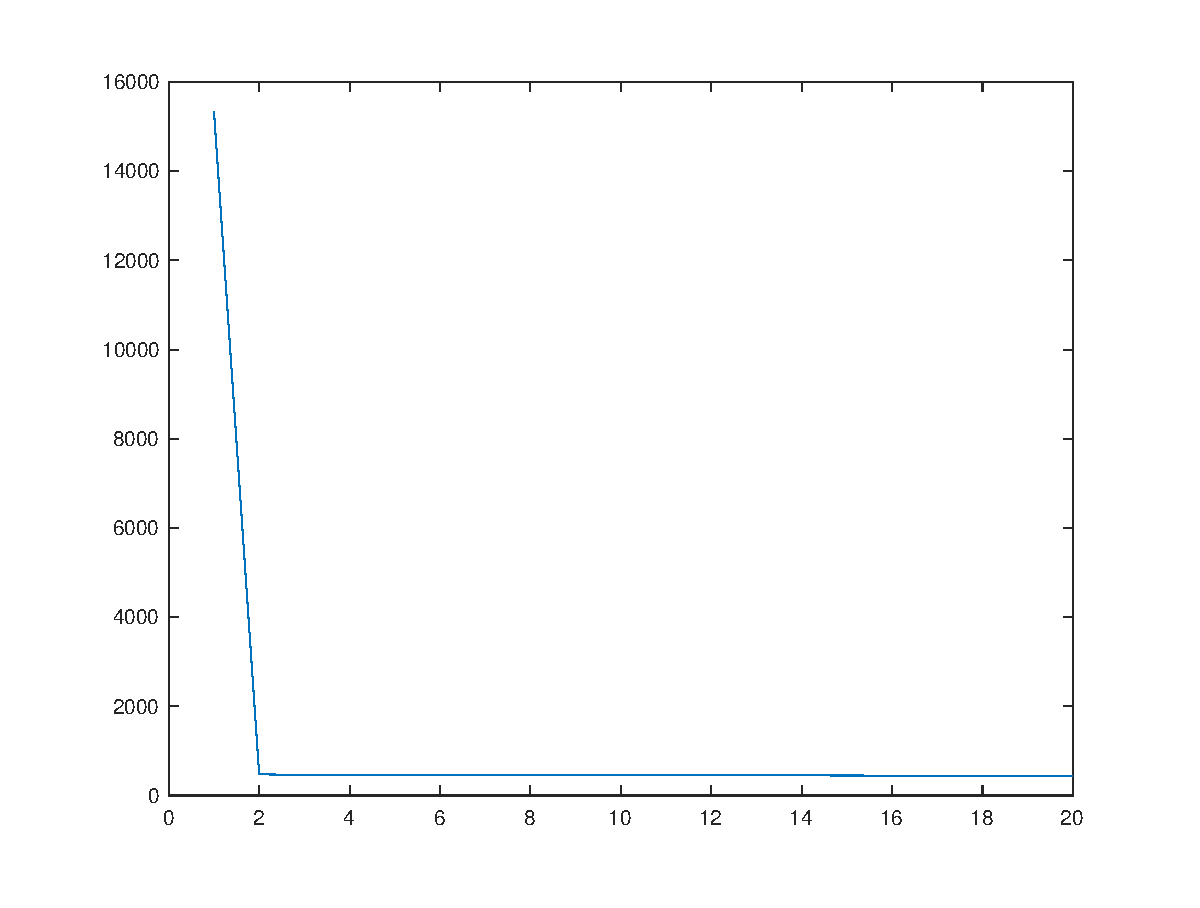
\includegraphics[width=3.5in]{cliffWANTEDa}
\caption{The type of 'cliff' drop-off in singular value magnitudes we wanted to see.}
\end{figure}

Unfortunately, the result was got did not have the sudden drop over just a few singular values.  What we got instead can be seen in \textbf{Figure \ref{fig:likes-cliffGOT}}.

\begin{figure}
\label{fig:likes-cliffGOT}
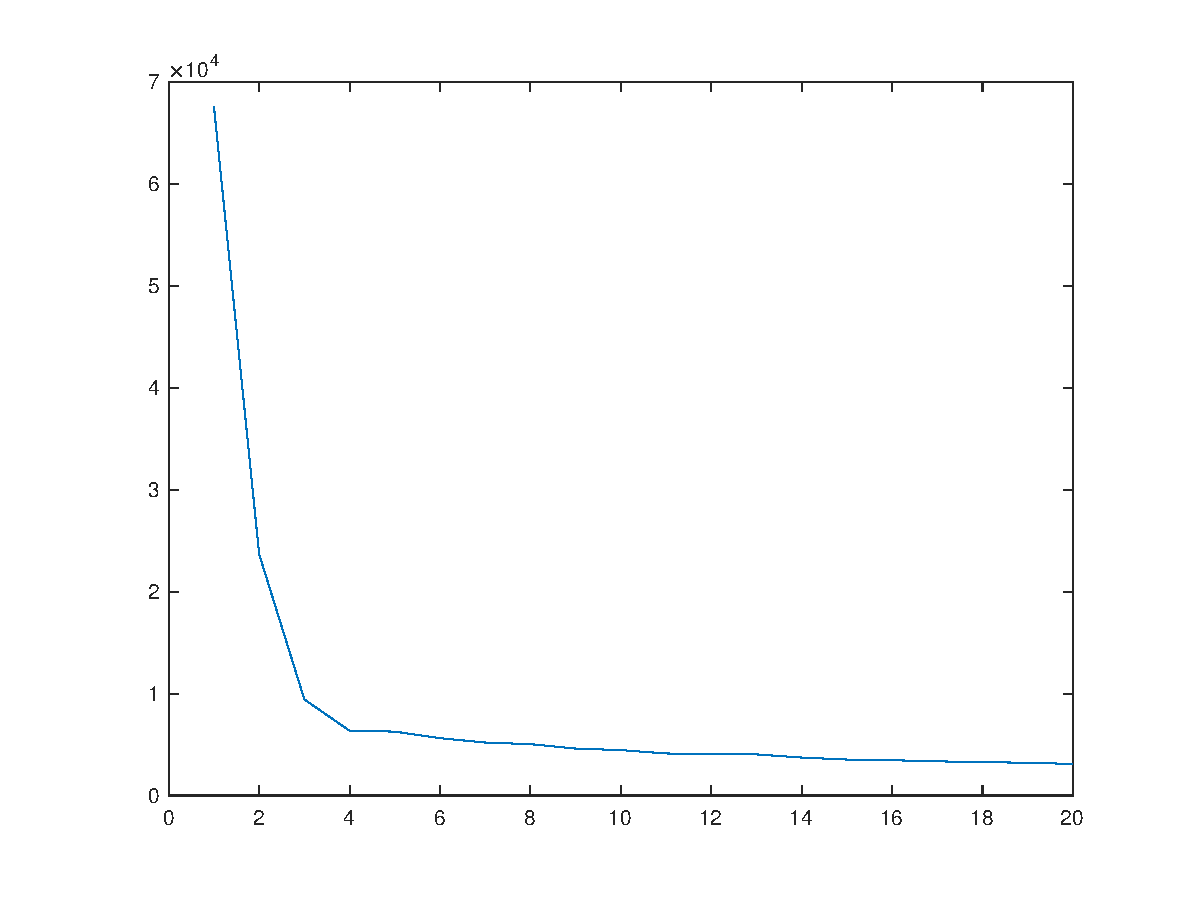
\includegraphics[width=3.5in]{cliffGOT}
\caption{The singular value magnitudes we got instead of what we wanted to see.}
\end{figure}



%---------------------------------------------------
%---------------------------------------------------



\section{Dataset and Metrics}

jklkjb






%---------------------------------------------------
%---------------------------------------------------


\section{Results}

kjgkjhg


%---------------------------------------------------

\subsection{Text}

For age prediction model, using Logistical regression based on 82-LIWC features is best choice in the method we tried. We also use other methods, line Linear regression, random forest, Na�ve Bayes. We can see the results in the chart given in \textbf{Table \ref{tab:txt-ageSEX}}.

\begin{table}
\caption{Text RESULTS for Age \& Gender Accuracy}
\label{tab:txt-ageSEX}
\begin{minipage}{\columnwidth}
	\begin{center}
	\begin{tabular}{l | c | c}
  		\toprule
   		Baseline				& 0.59						& 0.59	\\
		\hline
		Linear Regression		& 0.52						& 0.60	\\
		\hline
		Random Forest			& 0.51						& 0.60	\\
		\hline
		Naive Bayes			& 0.49						& 0.71	\\
		\hline
		Logistical Regression	& 0.61\footnote{Using LIWC data}	& 0.59	\\
							& 0.59\footnote{Using text data}	& 		\\
	\bottomrule
	\end{tabular}
	\end{center}
\bigskip
\end{minipage}	
\end{table}

From the chart in \textbf{Table \ref{tab:txt-ageSEX}}, we can see that the best result in age prediction is the model when it uses logistical regression based on LIWC, and the best accuracy in gender predict model is Na�ve Bayes. Therefore, our choice are Na�ve Bayes based on text in gender and Logistical Regression based on LIWC in age prediction.

For Big five personality, we only use linear regression on the text and LIWC part, because we tried other methods, and the results are same. The results are in the chart given in \textbf{Table tab:txt-person}

\begin{table}
\caption{Text RESULTS for Personality Score RMSE}
\label{tab:txt-person}
\begin{minipage}{\columnwidth}
	\begin{center}
	\begin{tabular}{l | c | c | c | c | c}
  	\toprule
						& \textbf{OPE}	& \textbf{NEU}	& \textbf{EXT}	& \textbf{AGR}	& \textbf{CON}	\\
		\hline
		Baseline			& 0.65		& 0.80		& 0.79		& 0.66		& 0.73		\\
		Linear Regression	& 0.65		& 0.79		& 0.79		& 0.65		& 0.72		\\
	\bottomrule
	\end{tabular}
	\end{center}
\bigskip
\end{minipage}
\end{table}

From the chart in \textbf{Table tab:txt-person}, we can clearly see that the results under the predict model are similar with Baseline when we use Linear regression.


%---------------------------------------------------

\subsection{Images}

jhlgjhg


%---------------------------------------------------

\subsection{Likes}

ljlkj



%---------------------------------------------------
%---------------------------------------------------


\section{Conclusion}

ljhgljhg


\subsection{Text}

For text part, we have tried many methods when we set up the model, but we do not have do more specific work on data preprocessing, such as feature selection, word choice. When we predict the age and gender, we can find more significant words, like she, he which will affect our results. Although we get a good result in the age prediction when we use Logistical regression based on 82 LIWC features, it is not perfect. In our last assignment, we find the neural network may be good at decrease RMSE in big five personality, thus we can try it in the future work. 


%---------------------------------------------------

\subsection{Images}

jbklj


%---------------------------------------------------

\subsection{Likes}

bljk







































































